\documentclass[10pt]{article}


% This is a helpful package that puts math inside length specifications
\usepackage{multirow}
\usepackage{wasysym}
\usepackage{marginnote}
\usepackage{url}
\usepackage{calc}
\usepackage[spanish, es-tabla]{babel}
\usepackage[utf8]{inputenc}
\usepackage{graphicx}
\usepackage{xcoffins}
\usepackage{array}
\usepackage{multicol}
\usepackage{multirow}
\usepackage{titlesec}
\usepackage[scaled=.90]{helvet}
\usepackage{fancyhdr}
\usepackage{markdown}
\usepackage[ddmmyyyy,hhmmss]{datetime}
\titleformat{\section}
  {\normalfont\sffamily\Large\bfseries\color{cyan}}
  {\thesection}{1em}{}

% Layout: Puts the section titles on left side of page
\reversemarginpar

%
%         PAPER SIZE, PAGE NUMBER, AND DOCUMENT LAYOUT NOTES:
%
% The next \usepackage line changes the layout for CV style section
% headings as marginal notes. It also sets up the paper size as either
% letter or A4. By default, letter was used. If A4 paper is desired,
% comment out the letterpaper lines and uncomment the a4paper lines.
%
% As you can see, the margin widths and section title widths can be
% easily adjusted.
%
% ALSO: Notice that the includefoot option can be commented OUT in order
% to put the PAGE NUMBER *IN* the bottom margin. This will make the
% effective text area larger.
%
% IF YOU WISH TO REMOVE THE ``of LASTPAGE'' next to each page number,
% see the note about the +LP and -LP lines below. Comment out the +LP
% and uncomment the -LP.
%
% IF YOU WISH TO REMOVE PAGE NUMBERS, be sure that the includefoot line
% is uncommented and ALSO uncomment the \pagestyle{empty} a few lines
% below.
%

%% Use these lines for letter-sized paper
\usepackage[paper=letterpaper,
            %includefoot, % Uncomment to put page number above margin
            marginparwidth=1.0in,     % Length of section titles
            marginparsep=.05in,       % Space between titles and text
            margin=1in,               % 1 inch margins
            includemp]{geometry}

%% Use these lines for A4-sized paper
%\usepackage[paper=a4paper,
%            %includefoot, % Uncomment to put page number above margin
%            marginparwidth=30.5mm,    % Length of section titles
%            marginparsep=1.5mm,       % Space between titles and text
%            margin=25mm,              % 25mm margins
%            includemp]{geometry}

%% More layout: Get rid of indenting throughout entire document
\setlength{\parindent}{0in}

%% This gives us fun enumeration environments. compactitem will be nice.
\usepackage{paralist}


%% Reference the last page in the page number
%
% NOTE: comment the +LP line and uncomment the -LP line to have page
%       numbers without the ``of ##'' last page reference)
%
% NOTE: uncomment the \pagestyle{empty} line to get rid of all page
%       numbers (make sure includefoot is commented out above)
%
\usepackage{fancyhdr,lastpage}
\pagestyle{fancy}
%\pagestyle{empty}      % Uncomment this to get rid of page numbers
\fancyhf{}\renewcommand{\headrulewidth}{0pt}
\fancyfootoffset{\marginparsep+\marginparwidth}
\newlength{\footpageshift}
\setlength{\footpageshift}
          {0.5\textwidth+0.5\marginparsep+0.5\marginparwidth-2in}
\lfoot{\hspace{\footpageshift}%
       \parbox{4in}{\, \hfill %
                    \arabic{page} / \protect\pageref*{LastPage} % +LP
%                    \arabic{page}                               % -LP
                    \hfill \,}}

% Finally, give us PDF bookmarks
\usepackage{color,hyperref}
\definecolor{darkblue}{rgb}{0.0,0.0,0.3}
\hypersetup{colorlinks,breaklinks,
            linkcolor=darkblue,urlcolor=darkblue,
            anchorcolor=darkblue,citecolor=darkblue}

%%%%%%%%%%%%%%%%%%%%%%%% End Document Setup %%%%%%%%%%%%%%%%%%%%%%%%%%%%


%%%%%%%%%%%%%%%%%%%%%%%%%%% Helper Commands %%%%%%%%%%%%%%%%%%%%%%%%%%%%

% The title (name) with a horizontal rule under it
%
% Usage: \makeheading{name}
%
% Place at top of document. It should be the first thing.
\newcommand{\makeheading}[1]%
        {\hspace*{-\marginparsep minus \marginparwidth}%
         \begin{minipage}[t]{\textwidth+\marginparwidth+\marginparsep}%
                {\large \bfseries #1}\\[-0.15\baselineskip]%
                 \rule{\columnwidth}{1pt}%
         \end{minipage}}

% The section headings
%
% Usage: \section{section name}
%
% Follow this section IMMEDIATELY with the first line of the section
% text. Do not put whitespace in between. That is, do this:
%
%       \section{My Information}
%       Here is my information.
%
% and NOT this:
%
%       \section{My Information}
%
%       Here is my information.
%
% Otherwise the top of the section header will not line up with the top
% of the section. Of course, using a single comment character (%) on
% empty lines allows for the function of the first example with the
% readability of the second example.
\renewcommand{\section}[2]%
        {\pagebreak[2]\vspace{1.3\baselineskip}%
         \phantomsection\addcontentsline{toc}{section}{#1}%
         \hspace{0in}%
         \marginpar{
         \raggedright \scshape #1}#2}

% An itemize-style list with lots of space between items
\newenvironment{outerlist}[1][\enskip\textbullet]%
        {\begin{itemize}[#1]}{\end{itemize}%
         \vspace{-.6\baselineskip}}

% An environment IDENTICAL to outerlist that has better pre-list spacing
% when used as the first thing in a \section 
\newenvironment{lonelist}[1][\enskip\textbullet]%
        {\vspace{-\baselineskip}\begin{list}{#1}{%
        \setlength{\partopsep}{0pt}%
        \setlength{\topsep}{0pt}}}
        {\end{list}\vspace{-.6\baselineskip}}

% An itemize-style list with little space between items
\newenvironment{innerlist}[1][\enskip\textbullet]%
        {\begin{compactitem}[#1]}{\end{compactitem}}

% To add some paragraph space between lines.
% This also tells LaTeX to preferably break a page on one of these gaps
% if there is a needed pagebreak nearby.
\newcommand{\blankline}{\quad\pagebreak[2]}

%%%%%%%%%%%%%%%%%%%%%%%% End Helper Commands %%%%%%%%%%%%%%%%%%%%%%%%%%%

%%%%%%%%%%%%%%%%%%%%%%%%% Begin CV Document %%%%%%%%%%%%%%%%%%%%%%%%%%%%

\newcolumntype{M}[1]{>{\centering\arraybackslash}m{#1}}
\newcolumntype{P}[1]{>{\hfill\arraybackslash}p{#1}}

\begin{document}
%{\sffamily 
%\marginnote{typeset text here...}
%{\fontfamily{cmss}\selectfont

\makeheading{\begin{tabular}{l P{40mm}}
  &  \textit{\footnotesize{Updated:}}   \\
Rodrigo Lopez-Farias, Ph.D. \footnotesize{\textit{Computer Science and Engineering}  } & \footnotesize{\textit{\today}}
\end{tabular}
}




\section{{Personal Information}}

\begin{tabular}{l P{55mm} M{10mm}}
Birthday: 8/Jul/984		&	e-mail:  rdglpz@gmail.com	& 
\multirow{2}{*}[0.3cm]{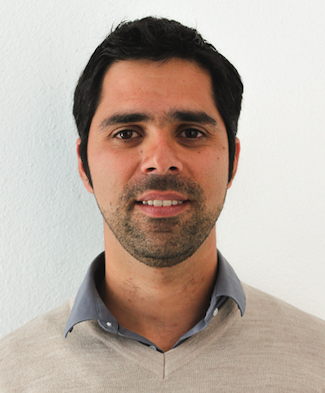
\includegraphics[width=2.0cm]{images/foto2017.png}  } 	\\
Residence: Corregidora, Queretaro  	&  Cellphone: +52 443 155 5416	 		&	\\
		& 	Skype ID: rdglpz  			&	\\
%\\       		&	ORCID ID: 0000-0003-2772-0051						&
& & \\
\end{tabular}


\blankline

\section{Current Job}
Associate researcher of the National Council on Science and Technology (CONACyT) commissioned and working at the Center for Research of Geo-spatial Information Sciences (CentroGeo) (Since Nov 2017).

\section{Grants and Distinctions}
Member of the Mexican System of Researchers (SNI) in the Candidate Category.
%Agentes conversacionales inteligentes manejando gran volumen de información (Big Data).

\blankline

\section{Interests \& Skills} \textbf{Programming and Data Base Managing Languages}

Python, R, Matlab, Mathematica, Java, C/C++, PHP-HTML-MySQL(SQL), CassandraDB (NoSQL, Cassandra Query Language).

\blankline

\textbf{Research}
   
Time and spatio-temporal (geographic information) series modelling and prediction with machine learning (Artificial Neural Networks, Nearest Neighbors, Support Vector Machines). Multi-Model Prediction with probabilistic model selection. Heuristics for global and non-convex optimization applied to System Identification in Biology Systems.
 
\blankline

\textbf{Research groups and projects}
\blankline

Network of Applied Computational Intelligence. \url{https://goo.gl/7B4RcE}.
Project of the Mexican Center of Energy Innovation in Electrical Power Systems: Forecasting the required natural resources for the production of renewable electric power. \url{https://www.ineel.mx/}.
\blankline
 
\textbf{Languages} 

English: 550 ITP TOEFL points. 

Italian: B1 Common CEFRL Level. 


\section{Academic Degree}  \textbf{Ph.D. in Computer Science and Engineering}. (With European Doctorate mention).

\textbf{Institute:} IMT School of Advanced Studies Lucca. Lucca, Italy. \textit{(Feb/2012 -  Jan/2016)}. 

\textbf{Thesis:} Time Series Forecasting Based on Classification of Dynamic Patterns.

\textbf{Advisors:} Ph.D. Alberto Bemporad. Ph.D. Pantelis Sopasakis.

\textbf{Field of study:} Time series analysis and modelling with machine learning.

\textbf{Taken Courses:} Semantics and formal methods. Algorithmic complexity. Basic linear algebra. Principles of parallel and concurrent computing. Performance modelling applied to Computer Networks. Specification, modelling and verification of reactive systems. Introduction to global and local optimization. Model checking. Optimum control,  (Optimization Algorithms). Programming Methodologies with Python. Cloud Computing. Theory of complex networks. Machine Learning. 

\blankline



\textbf{M.Sc. in Electrical Engineering (Computer Systems Group)}.

\textbf{University}: Michoacan University of San Nicolas de Hidalgo. (Universidad Michoacana de San Nicolas de Hidalgo). Morelia, Mexico. \textit{(Mar/2008 - Aug/2010)}.

\textbf{Thesis:} Bifurcation Diagrams for Discontinuous or Non-differentiable Equations.

\textbf{Advisors:}  Ph.D. Juan Jose Flores Romero, Ph.D. Claudio Fuerte E.

\textbf{Field of study:}  Evolutionary computing, unconstrained global optimization, nonlinear dynamical systems, stability analysis.

\blankline

\textbf{B.Eng. in Computer Systems}.

%Instituto Tecnológico de Morelia. Morelia, Mexico. \textit{(2002 2007)}.
\textbf{Institute:} Morelia Institute of Technology (Instituto Tecnológico de Morelia). Morelia, Mexico. \textit{(2002-2007)}.


\textbf{Thesis:} Implementation and performance analysis of \textbf{``Linux Terminal Server Project"} for educational purposes.

\textbf{Field of Study:} Applications of distributed operative systems.

\section{Academic Experience}  \textbf{Teaching}.

\blankline

\textbf{Queretaro Institute of Technology}. Queretaro, Mexico.

\begin{innerlist}
\item Internet of things (Computer Systems Engineering). \textit{(Jan/2020 - May/2020)}.
\end{innerlist}

\blankline

\textbf{Morelia Institute of Technology}. Morelia, Mexico.

\begin{innerlist}
\item Programming (Electrical Engineering), Programming and Algorithms (Mechanical Engineering), Algorithms and Programming Languages (Industrial Engineering), Operative Systems II (Engineering Informatics)), Programming II (Electronic Engineering). \textit{(Aug/2011  - Jan/2012)}.
\item Data structure and Organization (Information and Communication Technologies Engineering),Database fundamentals (Computer Systems Engineering) and Evaluation of software projects (Engineering Informatics). \textit{(Jan/2011 - Jul/2011)}.
\item Operative systems, selected topics of programming and research fundamentals(Computer Systems Engineering). \textit{(Aug/2010 - Dec/2010)}.
\end{innerlist}


\blankline

\blankline
\textbf{University of Morelia (Universidad de Morelia)}. Morelia, Mexico.

\begin{innerlist}
\item Web programming with PHP. \textit{(Aug/2009 - Dec/2009)}.
\end{innerlist}

\blankline

\section{Professional Experience}


%\textbf{Research Center and Advanced Studies of the Polytechnic National Institute}. (Nov/2016 - Current)


%\textbf{Department:} Coordination of Information and Communication Technology Services.

%\textbf{Activity:} Innovation and development of intelligent conversational agents for commercial purposes 

\blankline

\textbf{Center for Research and Advanced Studies of the National Polytechnic Institute (CINVESTAV)}

\textbf{Department:} Coordination and administration of Information and Communication Technologies Services (CGSTIC)

\textbf{Activity}: Application of machine learning algorithms for commercial conversational agents.
Mexico City. (Oct/2016 - July/2017).

\blankline

\textbf{Michoacan University of San Nicolas de Hidalgo}. (Oct/2015 - Oct/2016)

\textbf{Department:} Computer Center and University Information processes.

\textbf{Activity:} Web manager, programmer and collaborator for decision making for an efficient administration of university information.

\blankline

%\subsection{Participation in Research Projects}
\textbf{Center for Information and Communications Technologies (CETIC)}. \textit{(Mar/2007 - Jun/2007)}.
Morelia, Mexico.

\textbf{Department:}Infrastructure department.

\textbf{Activity:} Professional training in the project Performance analysis of \textbf{Linux Terminal Server Project} applied to to basic education.

\blankline

{\textbf{Morelia Institute of Technology}}. Morelia, Mexico. \textit{(Feb/2007)}

\textbf{Activity}: Social Service Project:  Web catalog with PHP for Social Service.

\blankline

%\textbf{IMPULSA}
%\blankline

%Participation in the young entrepreneurs program: IMPULSA.


%\blankline

\section{Publications} \textbf{Articles in Journals included in Journal Citation Reports}

\blankline


\textbf{Accepted}

%\subsection{Journal Articles Sent}
\begin{innerlist}

\item \textbf{Spatio-temporal Networks of light pollution} \textit{{Pichardo Corpus, Juan. A. and Solano-Lamphar, Hector and Lopez-Farias, Rodrigo, Delgadillo-Ruiz, Olivia}}. {Journal of Quantitative Spectroscopy and Radiative Transfer}. (doi: pending) ({June/2020}).

\item \textbf{Soft Computing Methods with Phase Space Reconstruction for Wind Speed Forecasting—A Performance Comparison} \textit{{Flores, Juan. J. and Cedeño González, José R. and Rodríguez, Héctor and Graff, Mario and Lopez-Farias, Rodrigo and Calderon, Felix}}. {Energies}. (doi: 0.3390/en12183545) ({Sept/2019}).

\item \textbf{Increasing weekend effect in ground-level O3 in metropolitan areas of Mexico} \textit{Iván Y. Hernández-Paniagua, Rodrigo Lopez-Farias, Jose J. Piña, Luis G. Ruíz-Suárez, Juan A. Pichardo-Corpus, Olivia Delgadillo, Agustín García-Reynoso, Arnoldo Flores-Torres, Alberto Mendoza}. {Sustainability}. (doi: 10.1109/ROPEC.2017.8261647) ({Aug/2018}).

\item \textbf{Multi-Model Prediction for Demand Forecast in
Water Distribution Networks} \textit{Rodrigo López Farías, Vicenc Puig, Héctor Rodriguez Rangel, Juan J. Flores} {Energies}. doi:10.3390/en11030660. ({Mar/2018}).

\item  \textbf{Evolving Nearest Neighbor Time Series Forecasters.} \textit{Juan J. Flores, José Cede\~no Gonzalez, Rodrigo López Farías, Félix Calderón }.  {Journal of Soft Computing},
DOI : 10.1007/s00500-017-2822-1. (Sept/2017).
%\item \textit{Juan J. Flores, Rodrigo López Farías, Julio Barrera, Carlos Coello }.  Performance of Gravitational Interaction Optimization Metaheuristics on High Dimensional Problems.  Enviado a  \textit{Journal of Metaheuristics, \url{https://goo.gl/6bZ4tE}, el 1 de Febrero 2017}.

\item \textbf{Short-Term Demand Forecast using Bank of Neural Network Models Trained using Genetic Algorithms for the Optimal Management of Drinking Water Networks.}\textit{Hector Rodriguez Rangel, Vicen\c{c} Puig, Rodrigo López Farías, Juan J. Flores.}  {Journal of Hydroinformatics}. DOI: 10.2166/hydro.2016.199. ISSN: 1464-7141 (Nov/2016).
%\item \textit{Juan J. Flores, Rodrigo López Farías, Julio Barrera, Carlos Coello }.  Performance of Gravitational Interaction Optimization Metaheuristics on High Dimensional Problems.  \textit{Journal of Metaheuristics}.(2016)
%\item \textit{Juan J. Flores, José Cede\~no Gonzalez, Rodrigo López Farías, Félix Calderón }.  Evolving Nearest Neighbor Time Series Forecasters. \textit{Journal of Time Series Analysis}.(2016)

\blankline

\textbf{Peer Reviewed Articles in Scientific and Technologic Divulgation Mexican Journals }


\blankline

\textbf{Accepted}

\begin{innerlist}


\item \textbf{Sistema de Medición de Flujos de Agua Tolerante a Fallos en Redes de Distribución de Agua Potable Utilizando Inteligencia Artificial}, \textit{H. Rodríguez Rangel, R. López Farías, G. Manjarrez Montelongo}, L. A. Morales Rosales y G. E. Peralta Peñuñuri. Komputer Sapiens, KS año 9 vol. 2, KS92, 2017, (Latin index).

\end{innerlist}

\blankline

\end{innerlist}

\blankline

\textbf{Peer Reviewed Accepted Articles in National and International Conferences}

\blankline
\textbf{Accepted}
\begin{innerlist}

\item \textbf{Automatic Modelling of Land Use Suitability Using Deep Feedforward Networks with Leon and
Silao, Guanajuato Region Data} \textit{Rodrigo López-Farías, Juan A. Pichardo-Corpus, Raúl A. Aguilar-Vilchis}. (ISSN: 2515-1762). {International Conference on Geospatial Information Sciences 2019}, \textbf{Merida, México, Oct/2019}. \url{http://bit.ly/2KHxelY}

\item \textbf{Adaptive Nearest Neighbors Phase Space Reconstruction for Short-Time Prediction in Chaotic Time Series} \textit{Rodrigo López-Farías, José R. Cedeño Gonzalez, Olivia Delgadillo Ruiz, Juan J. Flores}. (ISBN-13: 9781941763957 ) .{The 10th International Multi-Conference on Complexity, Informatics and Cybernetics}, \textbf{Orlando, USA, March/2019}.


\item \textbf{Parameter Identification and Qualitative Analysis with Differential Evolution of the Calcium Standard Kinetics Model} \textit{Norma C. Perez-Rosas, Rodrigo López-Farías, Agustín Guerrero-Hernández and Juan J. Flores}. (DOI: 10.1109/ROPEC.2017.8261647) .{IEEE Autumn Meeting on Power, Electronics and Computing}, \textbf{Ixtapa México, Nov/2017}.


\item \textbf{Comparison of Time Series Forecasting Techniques with respect to Tolerance to Noise.} \textit{Juan J. Flores, Felix Calderon Solorio, Jose Rafael Cede\~no Gonzalez, Jose Ortiz Bejar and Rodrigo Lopez Farias}. (Pendiente) .\textit{IEEE Autumn Meeting on Power, Electronics and Computing}, \textbf{Ixtapa Mexico, Nov/2016}.


\item \textbf{Holt-Winters Residual Modelling using an ANN trained by GA and Time Series Validation Applied to Water Demand Forecasting} \textit{Hector Rodriguez-Rangel, Vicen\c{c} Puig, Juan J. Flores and ,  Rodrigo López} Farías.. (Pending). \textbf{3rd International Conference on Control and Fault-Tolerant Systems} \textbf{Barcelona, Spain. Sept/2016}.

\item \textbf{Flow meter Data Validation and Reconstruction using Neural Networks: Application to the Barcelona Water Network} \textit{Hector Rodriguez Rangel, Vicen\c{c} Puig,Juan J. Flores and ,  Rodrigo López Farías.}. \url{https://goo.gl/i7muz7}. \textbf{2016 European Control Conference, Aalborg. June/2016}.

\item \textbf{Qualitative and Quantitative Mul} \textit{Rodrigo López Farías, Juan J. Flores and Vicen\c{c} Puig}.  ti-Model Forecasting with Nonlinear Noise Filter Applied to Water Demand \textit{IEEE Autumn Meeting on Power, Electronics and Computing}. DOI: 10.1109/ROPEC.2015.7395122.  \textbf{Ixtapa Mexico, Nov/2015}.

\item \textbf{FNN a Fuzzy Version of the Nearest Neighbour Time Series Forecasting Technique } \textit{Juan J. Flores, Jose Ortiz Bejar, Jose Rafael Cedeño, Carlos Lara-Alvarez and Rodrigo López Farías}. \textit{IEEE Autumn Meeting on Power, Electronics and Computing}. DOI: 10.1109/ROPEC.2015.7395125. \textbf{Ixtapa Mexico, Nov/2015 }.

\item \textbf{A Multiple-Model Predictor Approach Based on an On-Line Mode Recognition with Application to Water Demand Forecasting} \textit{Rodrigo López Farías, Vicen\c{c} Puig}.  \textit{International work-conference on Time Series 1. 
} URI https://goo.gl/njWQ1e. \textbf{Granada Spain, Jul/2015}.

\item \textbf{An implementation of a multi-model predictor based on the qualitative and quantitative decomposition of the time-series.} \textit{Rodrigo. López, Vicen\c{c} Puig, Hector Rodriguez.} URI http: //hdl.handle.net/2117/81862. \textit{International work-conference on Time Series 1 
} \textbf{Granada Spain, Jul/015}.

\item \textbf{Optimization with gravitational Interactions} \textit{Dr, Juan Flores, Rodrigo López, Julio Barrera.}   \textit{ROPEC XIII: Autumn Meeting of Electric power systems, electronic and computation ( Reunión de Oto\~no de Potencia, Electronica y Computacion)} \textbf{ Morelia Mexico, November 2011}.

\item \textbf{Gravitational Interactions Optimization.} Juan Flores, Rodrigo Lopez, Julio Barrera.  \textit{Learning and Intelligent OptimizatioN}  (LION 5) DOI 10.1007/978-3-642-25566-3\_17. \textbf{Rome, Italy - Jan/2011}. 

\item \textbf{Particle swarm optimization with gravitational interactions for multimodal and unimodal problems.} Juan J. Flores, Rodrigo Lopez and July Barrera.  In \textit{Proceedings of the 9th Mexican International Conference on Artificial Intelligence (MICAI 2010)}, pages 3361-370. Springer-Verlag. DOI 10.1007/978-3-642-16773-7\_31. \textbf{Pachuca, Mexico. November/2010.}

\end{innerlist}

\blankline





\section{Conferences, Seminars \& Workshops } \textbf{Given} \begin{innerlist}

\item $4^{th}$ National Seminar of machine learning and computational intelligence organized by the National Institute of Optics, Astrophysics and electronic. (SNAIC: Seminario Nacional de Aprendizaje 
e Inteligencia Computacional del Instituto Nacional de Astrofísica, Óptica y Electrónica, INAOE ). Water demand prediction with Genetic Algorithms for the optimum operation of the drinking water distribution system: the Barcelona Case. Michoacan University of San Nicolas de Hidalgo (Universidad Michoacana de San Nicolás de Hidalgo). (Morelia, Mexico. Sept/2016).

%\item 11$^{th}$ State Science and Innovation Congress (Congreso Estatal de Ciencia, Tecnologíae Innovación). Solving the Maximum Edge Weight Clique Problem Using Ant Colony Optimization\textbf{Morelia, Mexico. October / 2016}.

%\item IV Seminario Nacional de Aprendizaje e Inteligencia Computacional (SNAIC). Predicción de la demanda de Agua con Algoritmos Genéticos para la optimización de la distribución de la Demanda de Agua en Redes de Agua Potable. Instituto Nacional de Astrofísica, Óptica y Electrónica. Universidad Michoacana de San Nicolás de Hidalgo. \textbf{Morelia, Mexico. Septiembre 2016}..



\item 11$^{th}$ State Science, Technology and Innovation congress in  Engineering and computer Science. PSO with Interactive Niches and Quasi-Newton Local Searches. Search the most connected Clique in a Weighted Graph with Ant Colony Optimization. {Morelia, México. Oct/2016}.


 \item 10$^{th}$ State Congress of Science Technology and Innovation in  Engineering and computer Science. PSO with Interactive Niches and Quasi-Newton Local Searches. {Morelia, Mexico. Sep/2015}.


\item Activities of the $10^{th}$ Anniversary of the Instituto Tecnológico Superior de Ciudad Hidalgo - ' Evolutionary computing applied to dynamical systems'.(Ciudad Hidalgo, Mexico. October 2010).
  %\item Activities of X Anniversary of the Instituto Tecnológico Superior de Ciudad Hidalgo - ' Evolutionary computing applied to dynamical systems'.(Ciudad Hidalgo, México. October 2010).
%\item Week of Research Projects FIE of the UMSNH - 'Gravitational Interactions Optimization ' ( Morelia, Mexico. June 2010 ).
\item Week of Research Projects FIE of the UMSNH - 'Gravitational Interactions Optimization ' ( Morelia, Mexico. Jun/2010 )
%\item Semana de Proyectos de Investigación de la Facultad de la UMSNH- 'Optimización con Interacciones Gravitacionales' \textbf{Morelia, Mexico. June 2010}.

\item Week of Research Projects FIE of the Michoacan University of San Nicolás de Hidalgo - - 'Bifurcation Diagrams using Artificial Intelligence Algorithms (Diagramas de Bifurcación Utilizando Herramientas de Inteligencia Artificia)' {Morelia, Mexico. Jun/2009}.
%\item Semana de Proyectos de Investigación de la Facultad de la UMSNH - 'Diagramas de Bifurcación Utilizando Herramientas de Inteligencia Artificial' \textbf{Morelia, Mexico. June 2009}.

\end{innerlist}

\blankline


\textbf{Attended}
\begin{innerlist}
\item 5th HYCON2 Ph.D. School on Control of Networked and Large-Scale Systems and the EFFINET Ph.D. School on Control of Drinking Water Networks  (Lucca Italy, (1-5)/Jul/2013)
\item Java workshop in the 2nd Week of Computation and Systems.  {Morelia, Mexico (2006).}
\item Analysis and Object Oriented Design using UML  (Morelia Mexico,  (8-12)/Aug/2011)

%\item Taller de Java en la 2da Semana de Sistemas y Computación (Morelia Mexico, 2006)
%\item Week of Systems and computation in the Instituto Tecnológico de Morelia. \textit{Morelia, Mexico (2006)}.
%\item 2da. Semana de Sistemas y Computaci\'on en el Instituto Tecnológico de Morelia (Morelia Mexico, 2006).	
%\item Week of Systems and computation in the Instituto Tecnológico de Morelia. \textit{Morelia, Mexico (2005).}
\end{innerlist}
%}
\end{document}




%%%%%%%%%%%%%%%%%%%%%%%%%% End CV Document %%%%%%%%%%%%%%%%%%%%%%%%%%%%%

%%%%%%%%%%%%%%%%%%%%%%%%%% Git Instructions %%%%%%%%%%%%%%%%%%%%%%%%%%%%
%cd /Users/rodrigolopez/rdglpzCV/rdglpzEngCV
%git add rdglpzCVEng.tex
%git add rdglpzCVEng.pdf
%git commit -m "Changes"
%git push origin master
%%%%%%%%%%%%%%%%%%%%%%%%%%%%%%%%%%%%%%%%%%%%%%%%%%%%%%%%%%%%%%%%%%%%%%%%%


